\documentclass[12pt]{report}
\usepackage{tikz}
\usepackage{parskip}
\usepackage{mathtools}
\usepackage{flexisym}
\usepackage{verbatim}
\usepackage{scrextend}

\newcounter{casenum}
\newenvironment{caseof}{\setcounter{casenum}{1}}{\vskip.5\baselineskip}
\newcommand{\case}[2]{\vskip.5\baselineskip\par\noindent {\bfseries Case \arabic{casenum}:} #1\\#2\addtocounter{casenum}{1}}


\begin{document}
\newcommand\tab[1][1cm]{\hspace*{#1}}

%title page
\author{Andre Gregoire}
\title{CIS770 Homework 6}
\maketitle

%problem 1
\textbf{Problem1}\newline
\begin{flushleft}
	Let there be a PDA \textit{M} that recognizes A $\diamond$ B. There are DFAs $M_A, M_B$ that recognize A and B respectively because A and B are regular.  We make a new start state where we push the start symbol onto our stack and transition to $q_A$ which represents the DFA that recognizes A ($M_A$) which will read in the word of A.  For every  symbol we read in A we push some symbol onto our stack.  The symbol doesn't matter as long as it is consistent/the same for symbols that are read in (i.e. push 'a' for all symbols).  Now we let the machine non deterministically choose what is the middle of the string by giving it the option of an $\epsilon$ -transition and move to the state of $q_B$, which represents the DFA that recognizes B ($M_B$)where for each symbol we read in we now pop a symbol from our stack.  If we reach the end of the string and the only thing left on the stack is our starting symbol we pop our starting symbol on an $\epsilon$ -transition and move to an accepting state, otherwise it is rejected.
	
	\begin{center}
		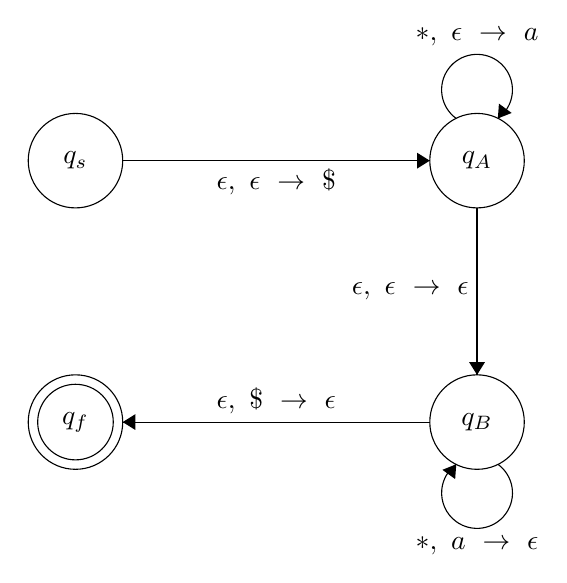
\begin{tikzpicture}[scale=0.2]
			\tikzstyle{every node}+=[inner sep=0pt]
			\draw [black] (9.4,-16.3) circle (3);
			\draw (9.4,-16.3) node {$q_s$};
			\draw [black] (34.9,-16.3) circle (3);
			\draw (34.9,-16.3) node {$q_A$};
			\draw [black] (34.9,-32.9) circle (3);
			\draw (34.9,-32.9) node {$q_B$};
			\draw [black] (9.4,-32.9) circle (3);
			\draw (9.4,-32.9) node {$q_f$};
			\draw [black] (9.4,-32.9) circle (2.4);
			\draw [black] (12.4,-16.3) -- (31.9,-16.3);
			\fill [black] (31.9,-16.3) -- (31.1,-15.8) -- (31.1,-16.8);
			\draw (22.15,-16.8) node [below] {$\epsilon,\mbox{ }\epsilon\mbox{ }\rightarrow\mbox{ }\$$};
			\draw [black] (34.9,-19.3) -- (34.9,-29.9);
			\fill [black] (34.9,-29.9) -- (35.4,-29.1) -- (34.4,-29.1);
			\draw (34.4,-24.6) node [left] {$\epsilon,\mbox{ }\epsilon\mbox{ }\rightarrow\mbox{ }\epsilon$};
			\draw [black] (31.9,-32.9) -- (12.4,-32.9);
			\fill [black] (12.4,-32.9) -- (13.2,-33.4) -- (13.2,-32.4);
			\draw (22.15,-32.4) node [above] {$\epsilon,\mbox{ }\$\mbox{ }\rightarrow\mbox{ }\epsilon$};
			\draw [black] (33.577,-13.62) arc (234:-54:2.25);
			\draw (34.9,-9.05) node [above] {$*,\mbox{ }\epsilon\mbox{ }\rightarrow\mbox{ }a$};
			\fill [black] (36.22,-13.62) -- (37.1,-13.27) -- (36.29,-12.68);
			\draw [black] (36.223,-35.58) arc (54:-234:2.25);w
			\draw (34.9,-40.15) node [below] {$*,\mbox{ }a\mbox{ }\rightarrow\mbox{ }\epsilon$};
			\fill [black] (33.58,-35.58) -- (32.7,-35.93) -- (33.51,-36.52);
		\end{tikzpicture}
	\end{center}
	
	{\footnotesize Note: The PDA above was just used to draw out my thoughts, the * symbol was used to denote any character in the alphabets of A and B}
\end{flushleft}

\pagebreak

M = (Q, $\Sigma$, $\Gamma$, $\delta$, $q_0$, F)
\begin{addmargin}[1cm]{0em}
	Q = \{$q_s, q_A, q_B, q_f$\}\\
	$\Sigma$ is the same for all\\
	$\Gamma$ = \{\$, a\}\\
	$\delta$(q,a,b)=$\begin{cases}
	\{q_A, \$\} &\text{if }q  = q_s, a = \epsilon, b = \epsilon\\
	\{q_A, a\} &\text{if }q  = q_A, a \in \Sigma, b = \epsilon\\
	\{q_B, \epsilon\} &\text{if }q  = q_s, a = \epsilon, b = \epsilon\\
	\{q_B, \epsilon\} &\text{if }q  = q_s, a \in \Sigma, b = 0\\
	\{q_f, \epsilon\} &\text{if }q  = q_s, a = \epsilon, b = \$\\
	\emptyset &otherwise\\
	\end{cases}$\\
	$q_0$ = $q_s$\\
	F = \{$q_f$\}\\
\end{addmargin}

\pagebreak
\textbf{Problem2}
\begin{flushleft}
	B = \{ \textit{w} $\vert$ \textit{w} is a palindrome made of \{0,1\}\textsuperscript{*} where the number of 0's and 1's are equal \}\\
	
	Given some  p (pumping length) we pick a word z $\in$ B such that $\vert$ z $\vert$ $\geq$ p.  Consider any division of z into \textit{u,v,w,x,y} such that $\vert$\textit{vwx}$\vert$ $\leq$ p and $\vert$ \textit{vx} $\vert$ $>$ 0\\
	
	A simple form for a palindrome word would be of the form ww\textsuperscript{R}\newline
	
	1) given \textit{p}\\
	2) z = 0\textsuperscript{p}1\textsuperscript{p}1\textsuperscript{p}0\textsuperscript{p}\\
	3) There are two cases to consider when splitting our chosen word \textit{z}.
	\begin{addmargin}[1cm]{0em}
		$\exists$ k $\geq$ 0. \textit{uv\textsuperscript{k}wx\textsuperscript{k}y} $\notin$ B\\
		Note: w = 0\textsuperscript{p}1\textsuperscript{p}, and w\textsuperscript{R} = 1\textsuperscript{p}0\textsuperscript{p}
		\begin{caseof}
			\case{\textit{vxy} contains only 1's}{ 0\textsuperscript{p}$\underbrace{1\textsuperscript{p}1\textsuperscript{p}}$0\textsuperscript{p}
				In this case if we pump the number of 1's will be different then the number of 0's. Thus \textit{z} $\notin$ B
			}
			\case{\textit{vxy} contains atleast one zero}{In the chosen word we can only contain zeros at the start or end of the string because of the constraint that $\vert$vxy$\vert$ $\leq$ p.  In this case there are two cases this could be true mentioned a moment ago.
				$\underbrace{0\textsuperscript{p}1\textsuperscript{p}}$1\textsuperscript{p}0\textsuperscript{p}, and
				0\textsuperscript{p}1\textsuperscript{p}$\underbrace{1\textsuperscript{p}0\textsuperscript{p}}$. There are three cases to account for depending on the the lengths of \textit{v} and \textit{x}.\\
			}
		\end{caseof}
		\begin{addmargin}[1cm]{0em}
			\begin{caseof}
				\case{0\textsuperscript{p+k}1\textsuperscript{p+k'}1\textsuperscript{p}0\textsuperscript{p}}{
					After pumping \textit{w}\textsuperscript{R} is not longer the reverse of \textit{w}. $\vert$\textit{w}$\vert$ $\neq$ $\vert$\textit{w}\textsuperscript{R}$\vert$\\   
					\textit{z} $\notin$ B\\
					}
				\case{0\textsuperscript{p}1\textsuperscript{p+k'}1\textsuperscript{p}0\textsuperscript{p}}{
					In this case, the $\vert$v$\vert$ = 0.  After pumping \textit{w}\textsuperscript{R} is not longer the reverse of \textit{w}. $\vert$\textit{w}$\vert$ $\neq$ $\vert$\textit{w}\textsuperscript{R}$\vert$\\
					\textit{z} $\notin$ B\\
					}
				\case{0\textsuperscript{p+k}1\textsuperscript{p}1\textsuperscript{p}0\textsuperscript{p}}{
					In this case, the $\vert$x$\vert$ = 0.  After pumping \textit{w}\textsuperscript{R} is not longer the reverse of \textit{w}. $\vert$\textit{w}$\vert$ $\neq$ $\vert$\textit{w}\textsuperscript{R}$\vert$\\
					\textit{z} $\notin$ B\\
					}
			\end{caseof}
		\end{addmargin}
	\end{addmargin}
	\pagebreak
	The cases are very similar for case 2 when we consider the opposite side, and the zero is contained from the end of the string rather than the beginning.\newline
	
	In both cases \textit{z} $\notin$ B thus B does not satisfy the pumping lemma showing it is not a context free language \\
\end{flushleft}


\pagebreak
\textbf{Problem3}
\begin{flushleft}
	A = \{ \textit{wtw}\textsuperscript{R} $\vert$ \textit{w, t} $\in$ \{0,1\}\textsuperscript{*} and $\vert$\textit{w}$\vert$ = $\vert$\textit{t}$\vert$  \}\\
	
	Given some  p (pumping length) we pick a word z $\in$ A such that $\vert$ z $\vert$ $\geq$ p.  Consider any division of z into \textit{u,v,w,x,y} such that $\vert$\textit{vwx}$\vert$ $\leq$ p and $\vert$ \textit{vx} $\vert$ $>$ 0\newline
	
	1) given \textit{p}\\
	2) z = 0\textsuperscript{p}1\textsuperscript{p}0\textsuperscript{p}\\
	3) There are two cases to consider when splitting our chosen word \textit{z}.
	\begin{addmargin}[1cm]{0em}
		$\exists$ k $\geq$ 0. \textit{uv\textsuperscript{k}wx\textsuperscript{k}y} $\notin$ A\\
		Note: \textit{w} = 0\textsuperscript{p}, \textit{t} = 1\textsuperscript{p}, \textit{w}\textsuperscript{R} = 0\textsuperscript{p}\\
		\begin{caseof}
			\case{\textit{vxy} contains only 1's}{0\textsuperscript{p}$\underbrace{1\textsuperscript{p}}$0\textsuperscript{p}
				In this case if we pump the number of 1's will be different then the number of 0's on the left side ($\vert$\textit{w}$\vert$ $\neq$ $\vert$\textit{t}$\vert$). 		Thus \textit{z} $\notin$ A
			}
			
			\case{\textit{vxy} contains atleast one zero}{In the chosen word we can only contain zeros at the start or end of the string because of the constraint that $\vert$vxy$\vert$ $\leq$ p.  In this case there are two cases this could be true mentioned a moment ago.
				0\textsuperscript{p}$\underbrace{1\textsuperscript{p}0\textsuperscript{p}}$ and 
				$\underbrace{0\textsuperscript{p}1\textsuperscript{p}}$0\textsuperscript{p}. 
				There are three more cases in this that vary depending on the lengths of \textit{v} and \textit{x}
			}
		\end{caseof}
		\begin{addmargin}[1cm]{0em}
			\begin{caseof}
				\case{0\textsuperscript{p+k}1\textsuperscript{p+k}0\textsuperscript{p}}{
					The right side of \textit{t} is no longer the reverse of the left side after pumping because $\vert$\textit{w}$\vert$ $\neq$ $\vert$\textit{w}\textsuperscript{R}$\vert$\\   
					\textit{z} $\notin$ A\\ 
					}
				\case{0\textsuperscript{p}1\textsuperscript{p+k}0\textsuperscript{p}}{
					$\vert$w$\vert$ $\neq$ $\vert$\textit{t}$\vert$ after pumping\\
					\textit{z} $\notin$ A\\ 
					}
				\case{0\textsuperscript{p+k}1\textsuperscript{p}0\textsuperscript{p}}{
					The right side of \textit{t} is no longer the reverse of the left side after pumping because $\vert$\textit{w}$\vert$ $\neq$ $\vert$\textit{w}\textsuperscript{R}$\vert$\\
					\textit{z} $\notin$ A\\ 
				}
			\end{caseof}
		\end{addmargin}
	\end{addmargin}
	
	\pagebreak
	The cases are very similar for case 2 when we consider the opposite side, and the zero is contained from the end of the string rather than the beginning.\newline

	In both cases \textit{z} $\notin$ A thus A does not satisfy the pumping lemma showing it is not a context free language 
\end{flushleft}

\end{document}
